
% =========================================================================================
% HOMEWORK TEMPLATE %===================================================================
% =========================================================================================

% =========================================================================================
% LaTeX SETUP %============================================================================
% =========================================================================================
\documentclass{report}						% Change "article" to "report" to get rid of page number on title page
\usepackage{amsmath,amsfonts,amsthm,amssymb,empheq}
\usepackage{setspace}
\usepackage{Tabbing}
\usepackage{fancyhdr}
\usepackage{lastpage}
\usepackage{extramarks}
\usepackage{chngpage}
\usepackage{soul,color}
\usepackage{graphicx,float,wrapfig}
\usepackage[retainorgcmds]{IEEEtrantools}

% =========================================================================================
% TikZ SETUP %==============================================================================
% =========================================================================================
\usepackage{tikz}
\usepackage{verbatim}
\usetikzlibrary{shapes,arrows,positioning,calc,scopes,angles,quotes}
\usetikzlibrary{decorations.markings}

% =========================================================================================
% MARGINS %===============================================================================
% =========================================================================================
\topmargin=-0.45in      
\evensidemargin=0in     
\oddsidemargin=0in      
\textwidth=6.5in        
\textheight=9.0in       
\headsep=0.25in         

% =========================================================================================
% ASSIGNMENT INFORMATION %===============================================================
% =========================================================================================
\newcommand{\hmwkTitle}{Homework\ \#4}
\newcommand{\hmwkDueDate}{ February\ 29,\ 2016}
\newcommand{\hmwkClass}{EE\ 324}
\newcommand{\hmwkClassTime}{Munk}
\newcommand{\hmwkClassInstructor}{Prof. Jens}
\newcommand{\hmwkAuthorName}{Blair Munro}

% =========================================================================================
% HEADER & FOOTER %=======================================================================
% =========================================================================================
\pagestyle{fancy}                                                       
\lhead{\hmwkAuthorName}                                                 
\chead{\hmwkClass\ (\hmwkClassInstructor\ \hmwkClassTime): \hmwkTitle}  
\rhead{\firstxmark}                                                     
\lfoot{\lastxmark}                                                      
\cfoot{}                                                                
\rfoot{Page\ \thepage\ of\ \pageref{LastPage}}                          
\renewcommand\headrulewidth{0.4pt}                                      
\renewcommand\footrulewidth{0.4pt}                                      

% =========================================================================================
% CUSTOM MATH COMMANDS %================================================================
% =========================================================================================
\newcommand{\ud}{\,\mathrm{d}}						%creates roman-script differential d , with added space
\newcommand{\pd}[2]{\frac {\partial #1}{\partial #2}} 										%partial derivative
\newcommand{\td}[2]{\frac {\mathrm{d} #1}{\mathrm{d} #2}}									  %derivative
\newcommand{\tdd}[2]{\frac {\mathrm{d}^2 #1}{\mathrm{d} #2^2}}  						      %second derivative
\newcommand{\val}[2]{#1 \text{ #2}}							 	    %formats a numerical value with text units
\newcommand{\comm}[1]{\text{#1}\qquad}
% =========================================================================================
% MAKE TITLE %=============================================================================
% =========================================================================================
\title{\vspace{2in}\textmd{\textbf{\hmwkClass:\ \hmwkTitle}}\\\normalsize\vspace{0.1in}\small{Due\ on\hmwkDueDate}\\\vspace{0.1in}\large{\textit{\hmwkClassInstructor\ \hmwkClassTime}}\vspace{3in}}
\date{}
\author{\textbf{\hmwkAuthorName}}

% =========================================================================================
% BEGIN DOCUMENT %=======================================================================
% =========================================================================================
\begin{document}
\begin{spacing}{1.1}
\maketitle

\newpage
\begin{enumerate}
%PROBLEMS ================================================================================
\item[{\bf \large 1.}] 
%	1
We have measured the following on a distortionless transmission line at 100 MHz:
\begin{align*}
Z_c&= 50\Omega\\
\alpha &= 1.15\times 10^{-3} \text{ (Nep/m)}\\
\beta &= 0.8\pi \text{ (rad/m)}
\end{align*}
Determine the per-length quantities $R_0$, $L_0$, $G_0$, and $C_0$.

The derivation of transmission line behavior results in two ordinary second order odes---the plain ol' one dimensional wave equation in spatial terms. These are:
	\begin{IEEEeqnarray*}{rCl}
	\tdd{I}{x}-\gamma^2I(x)&=&0\\
	\tdd{V}{x}-\gamma^2V(x)&=&0\\
	\end{IEEEeqnarray*}
and the proportionality constant in this case happens to be \[\gamma =\sqrt{(j\omega L_0+R_0)(j\omega C_0+G_0)}\]
Now, since any number can be expressed in terms of a real and an imaginary part, we therefore wish to express $\gamma$ as \[\gamma =\alpha+j\beta=\sqrt{(j\omega L_0+R_0)(j\omega C_0+G_0)}\]
To make things even better, we happen to be brilliant students who know that distortionless transmission lines represent a special case: That wherein the characteristic impedance is the root of per-unit inductance over capacitance! 
	\[Z_c=\sqrt{\frac{L_0}{C_0}}\]
Also, after insisting that $\beta$ be a linear function of $\omega$ the distortionless transmission line case also implies that 
	\[\gamma=\sqrt{\frac{L_0}{C_0}}R_0+j\omega\sqrt{L_0C_0}\]
Taking the real part of $\gamma$ equal to our experimentally determined propagation constant $\beta$, plus the characteristic impedance equation above, gives us a mighty convenient system of two equations with two unknowns. Solving,
	\begin{IEEEeqnarray*}{lrCl}
	\comm{plugging}&\beta&=&\omega\sqrt{L_0C_0}\\
	\comm{into}&Z_c&=&\sqrt{\frac{L_0}{C_0}}\\
	\comm{gives}&Z_c\beta&=&\omega\sqrt{\frac{L_0}{C_0}}\sqrt{L_0C_0}\\
	&&=&\omega L_0\\
	\comm{rearranging gives}&L_0&=&\frac{Z_c\beta}{\omega}\\
	\end{IEEEeqnarray*}
thus
	\[\boxed{L_0=\val{0.2}{$\frac{\mu\text{H}}{\text{m}}$}}\]
And the rest goes without showing:
	\[\boxed{C_0=\val{80}{$\frac{p\text{F}}{\text{m}}$}\text{, }R_0=\val{20}{$\frac{\mu\Omega}{\text{m}}$}\text{, }G_0=		\val{8}{$\frac{n\text{S}}{\text{m}}$}}\]
\item[{\bf \large 2.}] 
%	2
A 2 meter lossless air-spaced transmission line having a characteristic impedance of 50 ohms is terminated with an impedance of $40 +j30 \Omega$ at an operating frequency of 200 MHz. Find the input impedance.
\begin{figure}[!hbp]
\centering
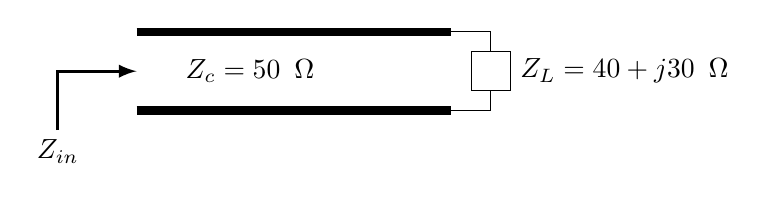
\begin{tikzpicture}[
	scale=1,
	vector/.style={very thick,->, >=latex},
	axis/.style={very thick, ->, >=stealth'}]
		\draw[line width=3pt] (0,1)--(4,1);
		\draw[line width=3pt] (0,0)--(4,0);
		\draw (4,1)--(4.5,1)--(4.5,0)--(4,0);
		\draw[fill=white] (4.25,0.75) rectangle (4.75,0.25);
		\draw (4.75,0.5) node[right]{$Z_L=40+j30\enspace\Omega$};
		\draw (0.5,0.5) node[right]{$Z_c=50\enspace\Omega$};
		\draw[vector] (-1,-0.25)|-(0,0.5);
		\draw (-1,-0.25) node[below]{$Z_{in}$};
\end{tikzpicture}
\caption{Problem 2, lossless transmission line in (effectively) free space.}
\end{figure}

At 200MHz in an air-spaced lossless transmission line, the wavelength will be $\lambda=1.5m$. This means the length of the transmission line is $\ell=\frac{4}{3}\lambda$. In this case, a Smith chart will be our friend...(see the next page):

First plot the normalized load impedance $Z_L=0.8+j0.6$ (in green)
After adjusting for the line length of 2 m, the new impedance is plotted by the yellow dot.
This unnormalized impedance of $z=0.67-j0.21$ is the answer:
\[\boxed{Z_{in}=33.5-j10.5\enspace\Omega}\]
\begin{figure}[!hbp]
\centering
\begin{tikzpicture}[
	scale=1,
	vector/.style={very thick,->, >=latex},
	axis/.style={very thick, ->, >=stealth'}]
		%	SMITH CHART: 
		%	2.34pt/mm	210pt, outer-mid	201pt, outer-inmid	225pt, outer	192pt, inner	
		%	[thick](90:226pt)--(90:238pt)		
		\node[inner sep=0pt] (russell) at (0,0){\includegraphics[width=1\textwidth]{SMITHCHARTSCAN.jpg}};
		\begin{scope}[shift={(-4pt,35.2pt)}]
			\draw[very thick, dashed, blue] (0,0)-- (89.5:225pt);
			\draw[very thick](89.5:226pt)--(89.5:238pt);
			\draw[very thick,dashed, red] (0,0) circle (64.35pt);
			\draw[fill=green] (89.5:64.35pt) circle (2pt);
			\draw[very thick, axis] (89.5:232pt) arc (89.5:89.5-360/3*8+3:232pt);
			\draw[very thick, axis] (89.5:232pt) arc (89.5:89.5-360/3*8-180:232pt);
			\draw[very thick, dashed, blue] (0,0)-- (-147:225pt);
			\draw[very thick](-147:226pt)--(-147:238pt);
			\draw[fill=yellow] (-147:64.35pt) circle (2pt);
			
		\end{scope}
\end{tikzpicture}
\caption{Smith Chart, Problem 2.}
\end{figure}
\newpage
%	3
\item[{\bf \large 3.}]
Consider, a $75\Omega$ transmission line terminated by a load impedance $Z_L=R_L+jX_L$. 
\begin{figure}[!hbp]
\centering
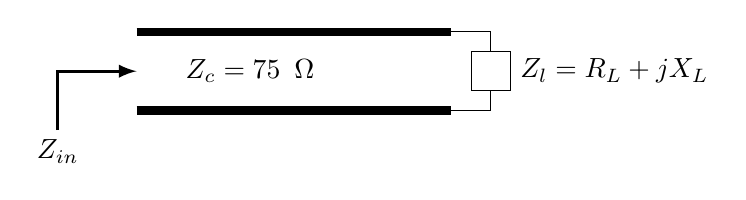
\begin{tikzpicture}[
	scale=1,
	vector/.style={very thick,->, >=latex},
	axis/.style={very thick, ->, >=stealth'}]
		\draw[line width=3pt] (0,1)--(4,1);
		\draw[line width=3pt] (0,0)--(4,0);
		\draw (4,1)--(4.5,1)--(4.5,0)--(4,0);
		\draw[fill=white] (4.25,0.75) rectangle (4.75,0.25);
		\draw (4.75,0.5) node[right]{$Z_l=R_L+jX_L$};
		\draw (0.5,0.5) node[right]{$Z_c=75\enspace\Omega$};
		\draw[vector] (-1,-0.25)|-(0,0.5);
		\draw (-1,-0.25) node[below]{$Z_{in}$};
\end{tikzpicture}
\caption{Problem 3, lossless transmission line in (effectively) free space.}
\end{figure}
\subitem{\bf\large (a)} Determine the relation between $R_L$ and $X_L$ that ensures a SWR of 3 on the line. this was tricky...I obviously wasn't understanding

So it is important to remember that $|\Gamma|$ is the modulus of a general complex number. We need to be very careful here and keep in mind that although we then define the function $\Gamma(x)=\Gamma e^{-j2\beta x}$, $\Gamma$ in this instance is \textit{still complex!} (I think us younglings have a tendency to assume that whenever we see a complex exponential tacked onto a symbol, that we are now in polar form. NO! LAZY BRAIN BAD!) Thus the actual $\Gamma$ magnitude is of some unknown combination of real part $\Gamma_{real}$ and imaginary $\Gamma_{imag}$. This is the reason for using a metric like SWR---it allows us to not worry about what exactly the real and imaginary parts of the reflection coefficient are if we don't need to. Ok, on with it:

\begin{IEEEeqnarray*}{rrCl}
\comm{First, we need to find the magnitude.}& SWR=3&=&\frac{1+|\Gamma|}{1-|\Gamma|}\\
&3-3|\Gamma|&=&1+|\Gamma|\\
&2&=&4|\Gamma|\\
\comm{thus Gamma is}& |\Gamma|&=& \frac{1}{2}\\
\end{IEEEeqnarray*}

And this checks out so far---a number between 1 and 0...

Now we exploit a boundary condition we know: The load impedance.
\begin{IEEEeqnarray*}{rrCl}
&Z_L&=&Z_c\frac{1+\Gamma}{1-\Gamma}\\
\comm{(complex here!)}&\Gamma&=&\frac{Z_L-Z_c}{Z_L+Z_c}\\
\comm{recognizing this, we now require}&|\Gamma|=\frac{1}{2}&=&\left|\frac{Z_L-Z_c}{Z_L+Z_c}\right|\\
&&=&\left|\frac{(R_L-R_c)+j(X_L-X_c)}{R_L+R_c)+j(X_L+X_c)}\right|\\
&&=&\frac{\sqrt{(R_L-R_c)^2+X_L^2}}{\sqrt{(R_L+R_c)^2+X_L^2}}\\
\comm{so}&\frac{1}{4}((R_L+R_c)^2+X_L^2)&=&((R_L-R_c)^2+X_L^2)\\
\comm{expanding}&\frac{1}{4}(R_L^2+2R_LR_c+R_c^2+X_L^2)&=&R_L^2-2R_LR_c+R_c^2+X_L^2\\
&\frac{3}{4}X_L^2&=&\frac{5}{2}R_LR_c-\frac{3}{4}R_L^2-\frac{3}{4}R_c^2\\
&X_L^2&=&\frac{10}{3}R_LR_c-R_L^2-R_c^2\\
\end{IEEEeqnarray*}

Thus \[\boxed{X_L=\sqrt{\frac{10}{3}R_LR_c-R_L^2-R_c^2}}\]

\subitem{\bf\large (b)} Find $X_L$ when $R_L=150\Omega$.

And so if we know $R_L$ must be 150 ohms, then it follows that to maintain a SWR of 3 we need a reactive load element \[\boxed{X_L=\val{96.8}{$\Omega$}}\]

This checks out too! A sanity check with at Smith Chart puts $Z_L=150+j96.8 \enspace\Omega$ at right where we need to be for a reflection coefficient of 0.5!

\subitem{\bf\large (c)} Find the voltage minimum in the line nearest to the load given the $Z_L$ from part (b).

I'm gunna use a Smith Chart. As we can see, the first minimum will occur at a point approximately\[\boxed{0.51\lambda \text{ away from the load}}\]
\begin{figure}[!hbp]
\centering
\begin{tikzpicture}[
	scale=1,
	vector/.style={very thick,->, >=latex},
	axis/.style={very thick, ->, >=stealth'}]
		%	SMITH CHART: 
		%	2.34pt/mm	210pt, outer-mid	201pt, outer-inmid	225pt, outer	192pt, inner	
		%	[thick](90:226pt)--(90:238pt)		
		\node[inner sep=0pt] (russell) at (0,0){\includegraphics[width=1\textwidth]{SMITHCHARTSCAN.jpg}};
		\begin{scope}[shift={(-4.8pt,35.2pt)}]
			\draw[axis, red, very thick, dashed] (29:41*2.34pt) arc(29:-180:41*2.34pt);
			\draw[dashed, red, very thick] (0,0)--(29:250pt);
			\draw[dashed, red, very thick] (0,0)--(-180:250pt);
			\draw[red] (-180:250pt) node [above right]{0.0};
			\draw[red] (29:250pt) node [above left]{0.21};
			\draw[fill=green] (180:41*2.34pt) circle(2pt);
			\draw[fill=green] (29:41*2.34pt) circle(2pt);
			
		\end{scope}
\end{tikzpicture}
\caption{Smith Chart, Problem 3c.}
\end{figure}
\newpage
%	4
\item[{\bf \large 4.}]
Normalized total impedance for a lossless transmission line is given by \[z(x)=\frac{1+\Gamma(x)}{1-\Gamma(x)},\] with \[\Gamma(x)=\Gamma_0e^{-j2\beta x},\]
and we can always express this normalized impedance in terms of a real and imaginary part, \[z(x)=r(x)+j\mathrm{x}(x).\]

\subitem{\bf\large (a)} Use MATLAB to plot the real and imaginary components of $\Gamma(x)$ over $-\infty<\mathrm{x}<\infty$ given $r$ values of 0, 0.25, 0.5, 1.0, 2.0, and 4.0.

\begin{figure}[!hbp]
\centering
\begin{tikzpicture}
		\node[inner sep=0pt] (russell) at (0,0){\includegraphics[width=1\textwidth]{4prob4a.jpg}};
\end{tikzpicture}
\caption{$r \in [0 \enspace0.25 \enspace0.5 \enspace1 \enspace2\enspace 4]\enspace \&\enspace X\in (-100,100)$}
\end{figure}
First use Euler's to get $\Gamma$ into rectangular form.
\begin{IEEEeqnarray*}{rrCl}
	&(r+jX)(1-\Gamma)&=&1+\Gamma\\
	&r-r\Gamma +jXr-j\Gamma X&=&1+\Gamma\\
	&r+jXr-1&=&\Gamma +r\Gamma +j\Gamma X\\
	&&=&\Gamma(1+r+jX)\\
	\comm{so}&\Gamma(x)=\frac{r-1+jXr}{r+1+jX}\\
\end{IEEEeqnarray*}

\subitem{\bf\large (b)} Do this again, but this time swap for the interval over $0 \leq r<  \infty$ and $\mathrm{x}$ values 0, $\pm$0.25, $\pm$0.5, $\pm$1.0, $\pm$2.0, $\pm$4.0.

\begin{figure}[!hbp]
\centering
\begin{tikzpicture}
		\node[inner sep=0pt] (russell) at (0,0){\includegraphics[width=1\textwidth]{4prob4b.png}};
\end{tikzpicture}
\caption{$X \in [0 \enspace\pm0.25 \enspace\pm0.5 \enspace\pm1 \enspace\pm2\enspace \pm4]\enspace \&\enspace r\in [0,10000)$}
\end{figure}

%	5
\item[{\bf \large 5.}]
A lossless transmission line has a characteristic impedance of 75 ohms. Use a Smith Chart to find the input impedance at 200MHz for the following two cases:

For both cases, the wavelength (assuming the transmission lines are air-spaced) is $\lambda=1.5\enspace \text{m}.$

\subitem{\bf\large (a)} A line that is 1.0m long, in open-circuit. In this case, the transmission line length $\ell$ in terms of the wavelength is $\ell=\frac{2}{3}\lambda$, or 0.666. 
\begin{figure}[!hbp]
\centering
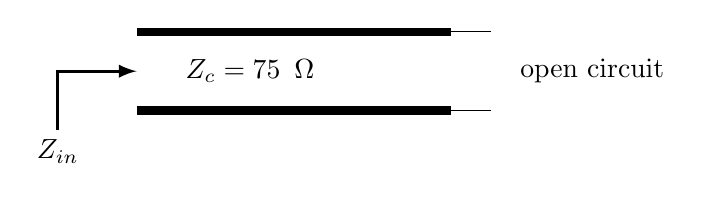
\begin{tikzpicture}[
	scale=1,
	vector/.style={very thick,->, >=latex},
	axis/.style={very thick, ->, >=stealth'}]
		\draw[line width=3pt] (0,1)--(4,1);
		\draw[line width=3pt] (0,0)--(4,0);
		\draw (4,1)--(4.5,1) (4.5,0)--(4,0);
		\draw (4.75,0.5) node[right]{open circuit};
		\draw (0.5,0.5) node[right]{$Z_c=75\enspace\Omega$};
		\draw[vector] (-1,-0.25)|-(0,0.5);
		\draw (-1,-0.25) node[below]{$Z_{in}$};
\end{tikzpicture}
\caption{Problem 5b, lossless transmission line in (effectively) free space, open circuit load.}
\end{figure}

\begin{figure}[!hbp]
\centering
\begin{tikzpicture}[
	scale=1,
	vector/.style={very thick,->, >=latex},
	axis/.style={very thick, ->, >=stealth'}]
		%	SMITH CHART: 
		%	2.34pt/mm	210pt, outer-mid	201pt, outer-inmid	225pt, outer	192pt, inner	
		%	[thick](90:226pt)--(90:238pt)		
		\node[inner sep=0pt] (russell) at (0,0){\includegraphics[width=1\textwidth]{SMITHCHARTSCAN.jpg}};
		\begin{scope}[shift={(-4.8pt,35.2pt)}]
			\draw[dashed, red, very thick] (0,0)--(0:250pt);
			\draw[red] (0:250pt) node [above]{0.251};
			\draw[fill=green] (0:192pt) circle(2pt);
			\draw[very thick, axis, dashed, red] (0:180pt) arc (0:-30:180pt);
			\draw[very thick, axis, dashed, red] (-30:180pt) arc (-30:-180:180pt);
			\draw[very thick, axis, dashed, red] (-180:180pt) arc (-180:-210:180pt);
			\draw[very thick, axis, dashed, red] (-210:180pt) arc (-210:-360:180pt);
			\draw[very thick, axis, dashed, red] (0:180pt) arc (0:-120:175pt);
			\draw[dashed, red, very thick] (0,0)--(-119:250pt);
			\draw[red] (-115:250pt) node [left]{0.416};
			\draw[fill=green](-119:192pt) circle (2pt);
		\end{scope}
\end{tikzpicture}
\caption{Smith Chart, problem 5a.}
\end{figure}
\newpage
So, by inspection, the non-normal input impedance must be \[\boxed{Z_{in}=-j44.25\Omega}\]

\subitem{\bf\large (b)} A line that is 0.8m long, in short-circuit.

\begin{figure}[!hbp]
\centering
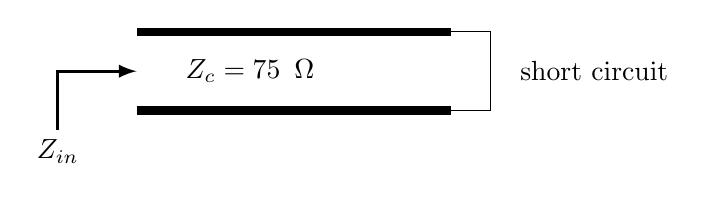
\begin{tikzpicture}[
	scale=1,
	vector/.style={very thick,->, >=latex},
	axis/.style={very thick, ->, >=stealth'}]
		\draw[line width=3pt] (0,1)--(4,1);
		\draw[line width=3pt] (0,0)--(4,0);
		\draw (4,1)--(4.5,1)--(4.5,0)--(4,0);
		\draw (4.75,0.5) node[right]{short circuit};
		\draw (0.5,0.5) node[right]{$Z_c=75\enspace\Omega$};
		\draw[vector] (-1,-0.25)|-(0,0.5);
		\draw (-1,-0.25) node[below]{$Z_{in}$};
\end{tikzpicture}
\caption{Problem 5b, lossless transmission line in (effectively) free space, short circuit load.}
\end{figure}

In this case, the transmission line length $\ell$ in terms of the wavelength is $\ell=\frac{8}{15}\lambda$, or 0.5333. 

\begin{figure}[!hbp]
\centering
\begin{tikzpicture}[
	scale=1,
	vector/.style={very thick,->, >=latex},
	axis/.style={very thick, ->, >=stealth'}]
		%	SMITH CHART: 
		%	2.34pt/mm	210pt, outer-mid	201pt, outer-inmid	225pt, outer	192pt, inner	
		%	[thick](90:226pt)--(90:238pt)	240pt, node
		\node[inner sep=0pt] (russell) at (0,0){\includegraphics[width=1\textwidth]{SMITHCHARTSCAN.jpg}};
		\begin{scope}[shift={(-4.8pt,35.2pt)}]
			\draw[very thick, dashed, red](0,0)--(-180:250pt);
			\draw[red] (-180:240pt) node [above]{0.499};
			\draw[fill=green] (-180:192pt) circle(2pt);
			\draw[very thick, axis, dashed, red] (-180:180pt) arc (-180:-210:180pt);
			\draw[very thick, axis, dashed, red] (-210:180pt) arc (-210:-360:180pt);
			\draw[very thick, axis, dashed, red] (-360:180pt) arc (-360:-390:180pt);
			\draw[very thick, axis, dashed, red] (-390:180pt) arc (-390:-540:175pt);
			\draw[very thick, axis, dashed, red] (-540:170pt) arc (-540:-564:175pt);
			\draw[very thick, dashed, red](0,0)--(-565:250pt);
			\draw[red] (-565:245pt) node [above]{0.034};
			\draw[fill=green] (-565:192pt) circle(2pt);
		\end{scope}
\end{tikzpicture}
\caption{Smith Chart, problem 5b.}
\end{figure}
$z_{in}=j0.225\Omega$ Thus the input impedance is \[\boxed{Z_{in}=j\val{16.88}{$\Omega$}}\]
\newpage
%	6
\item[{\bf \large 6.}]
A lossless transmission line that is $0.101\lambda$ long has a characteristic impedance of 50 ohms and is terminated by a $30-j10\Omega$. 
\begin{figure}[!hbp]
\centering
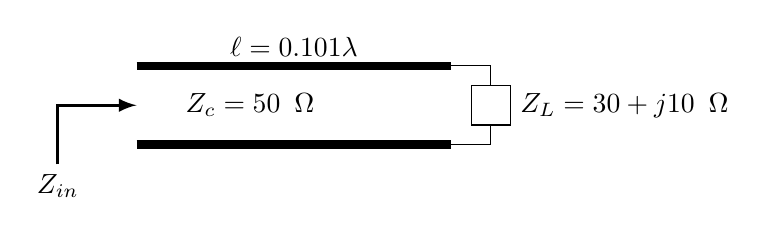
\begin{tikzpicture}[
	scale=1,
	vector/.style={very thick,->, >=latex},
	axis/.style={very thick, ->, >=stealth'}]
		\draw[line width=3pt] (0,1)--(4,1);
		\draw[line width=3pt] (0,0)--(4,0);
		\draw (4,1)--(4.5,1)--(4.5,0)--(4,0);
		\draw[fill=white] (4.25,0.75) rectangle (4.75,0.25);
		\draw (4.75,0.5) node[right]{$Z_L=30+j10\enspace\Omega$};
		\draw (0.5,0.5) node[right]{$Z_c=50\enspace\Omega$};
		\draw[vector] (-1,-0.25)|-(0,0.5);
		\draw (-1,-0.25) node[below]{$Z_{in}$};
		\draw (2,1) node[above]{$\ell=0.101\lambda$};
\end{tikzpicture}
\caption{Problem 2, lossless transmission line in (effectively) free space.}
\end{figure}

Using a Smith Chart, find the following:
\subitem{\bf\large (a)} Standing wave ratio (SWR)
\[\boxed{\text{SWR}=1.8}\]
\subitem{\bf\large (b)} The amplitude and phase angle of the voltage reflection coefficient
\[\boxed{\Gamma_L=0.28\angle145.4^\circ}\]
\subitem{\bf\large (c)} The input impedance
\[\boxed{Z_{in}=55+j29\enspace\Omega}\]
\subitem{\bf\large (d)} The location of the first voltage minimum in the line.
First minimum occurs \[\boxed{0.048\lambda \text{ away from the load}}\]
\begin{figure}[!hbp]
\centering
\begin{tikzpicture}[
	scale=1,
	vector/.style={very thick,->, >=latex},
	axis/.style={very thick, ->, >=stealth'}]

		%	SMITH CHART: 
		%	2.34pt/mm	210pt, outer-mid	201pt, outer-inmid	225pt, outer	192pt, inner	
		%	[thick](90:226pt)--(90:238pt)		
		\node[inner sep=0pt] (russell) at (0,0){\includegraphics[width=1\textwidth]{SMITHCHARTSCAN.jpg}};
		\begin{scope}[shift={(-4.8pt,35.2pt)}]
			\draw[dashed, red, very thick] (0,0)--(-145.5:250pt);
			\draw[red] (-145.5:250pt) node [below right]{0.452};
			\draw[fill=green] (-145.5:53.5pt) circle(2pt);
			\draw[very thick, purple, axis] (0,0)--(0:53.5pt);
			\draw[purple](0:27pt) node[above]{SWR} (0:27pt) node[below]{1.8};
			\draw[very thick, blue, axis,shift={(-6.7,-10.35)}] (0,0)--(0:53.5pt);
			\draw[blue](-5.7,-10.35) node[above]{$\Gamma_L$};
			\draw[blue](-5.7,-10.35) node[below]{$0.28$};
			\draw[axis,red](0:15pt)arc(0:-145:15pt) ;
			\draw[red](-90:15pt) node[below]{$\angle\Gamma_L$};
			\draw[red] (-90:25pt) node[below]{$145.5^\circ$};
			\draw[dashed, red, very thick] (0,0)--(71.3:250pt);
			\draw[dashed, red, very thick, axis] (-145.5:180pt) arc (-145.5:-360+71.3:180pt);
			\draw[red] (71.3:250pt) node [right]{0.351};
			\draw[fill=green] (71.3:53.5pt) circle (2pt);
			\draw (71.3:53.6pt)--(45:280pt);
			\draw(45:280pt) node[above right]{$z=\val{1.1+$j$0.58}{$\Omega$}$};
			\draw(45:280pt) node[below right]{$Z_{in}=\val{55+$j$29}{$\Omega$}$};
			\draw[very thick, blue] (0,0)--(-180:250pt);
			\draw[blue](-180:125pt) node[above]{V minimum};
			\draw[blue, very thick, dashed, axis] (-145.4:240pt) arc(-145.4:-180:240pt);
			\draw[blue] (-167:240pt) node [right]{$\Delta\ell=0.048\lambda$};
			\draw[blue] (-170:240pt) node [right]{V min occurs at};

			
		\end{scope}
\end{tikzpicture}
\caption{Smith Chart}
\end{figure}
\newpage
%	7
\item[{\bf \large 7.}]
Say we are doing a lab experiment on a 75 ohm lossless transmission line that is terminated by an unknown load impedance. If we find that the SWR is 3, and the successive voltage minima are 25cm apart (with the first occuring 10cm from the load) then determine the following:
\begin{figure}[!hbp]
\centering
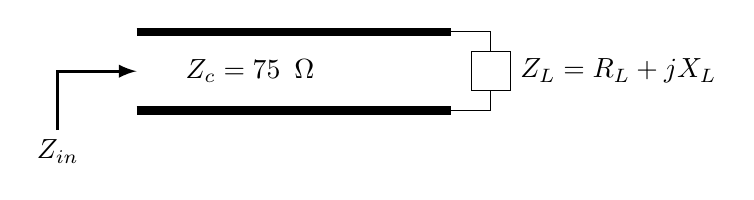
\begin{tikzpicture}[
	scale=1,
	vector/.style={very thick,->, >=latex},
	axis/.style={very thick, ->, >=stealth'}]
		\draw[line width=3pt] (0,1)--(4,1);
		\draw[line width=3pt] (0,0)--(4,0);
		\draw (4,1)--(4.5,1)--(4.5,0)--(4,0);
		\draw[fill=white] (4.25,0.75) rectangle (4.75,0.25);
		\draw (4.75,0.5) node[right]{$Z_L=R_L+jX_L$};
		\draw (0.5,0.5) node[right]{$Z_c=75\enspace\Omega$};
		\draw[vector] (-1,-0.25)|-(0,0.5);
		\draw (-1,-0.25) node[below]{$Z_{in}$};
\end{tikzpicture}
\caption{Problem 3, lossless transmission line in (effectively) free space.}
\end{figure}

So right off the bat, we know that the wavelength of the signal we are working with is 25cm.

We can take it a step further too---if the first minimum is 10cm from the load, we know the load is therefore $0.4\lambda$ wavelengths away, and this gives us a nice place to start on the Smith Chart.
\subitem{\bf\large (a)} The unknown load impedance.
\[\boxed{Z_L=25.5+j30.5\enspace\Omega}\]
\subitem{\bf\large (b)} The reflection coefficient at the load.
\[\boxed{\Gamma_L=0.5\angle108^\circ}\]
\subitem{\bf\large (c)} Where the first voltage minimum would occur if the load were replaced by a short.
\newline\newline\boxed{\text{This is a trick question. The voltage would be a minimum at the load if it were replaced by a short.}}
\end{enumerate}

\begin{figure}[!hbp]
\centering
\begin{tikzpicture}[
	scale=1,
	vector/.style={very thick,->, >=latex},
	axis/.style={very thick, ->, >=stealth'}]
		%	SMITH CHART: 
		%	2.34pt/mm	210pt, outer-mid	201pt, outer-inmid	225pt, outer	192pt, inner	
		%	[thick](90:226pt)--(90:238pt)		
		\node[inner sep=0pt] (russell) at (0,0){\includegraphics[width=1\textwidth]{SMITHCHARTSCAN.jpg}};
		\begin{scope}[shift={(-4.8pt,35.2pt)}]
			\draw[red, very thick, dashed] (0,0)--(-180:180pt);
			\draw[axis, red, very thick, dashed] (-180:180pt) arc(-180:108:180pt);
			\draw[red, very thick, dashed](0,0)--(108:250pt);
			\draw[red] (108:250pt) node [right]{0.099};
			\draw[very thick, purple, axis] (0,0)--(0:96pt); 
			\draw[purple](0:47pt)node[above]{SWR$=3$}; 
			\draw[very thick, dashed, purple, axis] (0:95pt) arc (0:108:95pt); 
			\draw[fill=green] (108:95pt) circle(2pt);
			\draw[very thick, orange, axis,shift={(-6.7,-10.37)}] (0,0)--(0:96pt);
			\draw[orange,shift={(-6.7,-10.37)}](0:45pt)node[below]{$\Gamma_L=0.5$};
			\draw[very thick,orange, axis] (0:15pt)arc(0:108:15pt);
			\draw[orange] (54:15pt)node[above right]{$\angle\Gamma_L=108^\circ$};
			\draw (108:97pt)--(80:270pt);
			\draw(80:270pt)node[above right]{$z=0.51+j0.61\enspace\Omega$};
			\draw(80:270pt)node[ below right]{$Z_L=25.5+j30.5\enspace\Omega$};
			
		\end{scope}
\end{tikzpicture}
\caption{Smith Chart}
\end{figure}

\end{spacing}

\end{document}




















